\section{Neural Network}

The CryptoNet project can be summarized in this graph:

\begin{figure}[H]
	\centering
	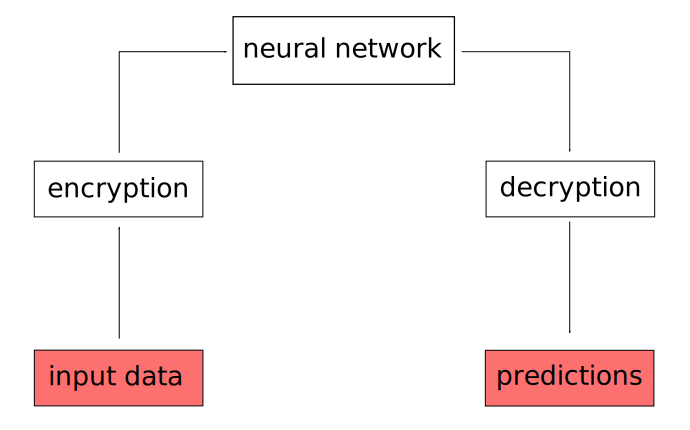
\includegraphics[width=0.8\textwidth]{images/fig2.pdf}
    \caption{The CryptoNets scheme.}
    \label{fig:im2}
\end{figure}

\noindent that is, it is a matter of applying a neural network to encrypted data to obtain encrypted predictions, and finally decrypt these to classify the initial input (image classification). But as we'll show, this scheme involves a simplification, ie it does not consider the process followed to obtain a model that can be applied to encrypted data. Below, we will analyze the problems that arise in the use of homomorphic cryptography techniques on neural networks, as well as other considerations regarding the network.

\subsection{The fundamental operations}

As we have shown in the Section 2, the only operations allowed by the homomorphic algorithm are the sum and the product. This partially limits the operations that can be performed by the network. Furthermore, it is important to remember that we are dealing with polynomials. In particular, in a neural network, a single neuron corresponds to the application of an activation function to the weighted sum of the outputs from neurons in the previous layer, to which is added a weight called bias:

\begin{equation*}
    y = f\left(\sum\limits_i w_i x_i + b\right)
\end{equation*}

\noindent with $x_i$ the previous outputs, $w_i$ the weights and $b$ the bias. But as said, the data to be manipulated are polynomials, and not simple scalar numbers. This means that we must consider every $x_i$ not as a single number, but as a polynomial, whose coefficients come from values of different images. So we can identify in the previous equation four different operations: the polynomial-scalar product, given by the multiplication of $x_i$ with $w_i$; the polynomial-polynomial sum, given by the sum of the single weighted polynomials; the polynomial-scalar sum, given by the sum of the resulting polynomial with the bias; and the activation function. The first two operations are straightforward, and they are obtained without the use of particular artifices (apart the reduction modulo $q$ of the coefficients). The polynomial-scalar product occurs simply by multiplying each of the single coefficients by the parameter $w_i$:

\begin{align*}
    &w_i(a_0+a_1x+a_2x^2+...+a_{n-1}x^{n-1}) =\\
    &\quad = w_ia_0+w_ia_1x+w_ia_2x^2+...+w_ia_{n-1}x^{n-1}
\end{align*}


This allows us, during the computation of the neural network, to momentarily neglect the fact that they are polynomials, and to treat each coefficient separately from the other, as in a normal neural network. The same applies to the polynomial-polynomial sum:

\begin{align*}
    &(a_0+a_1x+...+a_{n-1}x^{n-1})+(b_0+b_1x+...+b_{n-1}x^{n-1}) =\\
    &\quad = (a_0+b_0)+(a_1+b_1)x+...+(a_{n-1}+b_{n-1})x^{n-1}
\end{align*}


The polynomial-scalar sum is more complicated. What we want to obtain is that every value included in the polynomial is treated in the same way, ie we would like to obtain an output given by the sum of the input polynomial and of another virtual polynomial constructed using the bias $b$ for all coefficients:

\begin{equation*}
    b+bx+bx^2+...+bx^{n-1}
\end{equation*}

But adding this polynomial would not give the desired result. This is due to the type of encoding used, ie CRT batching. In particular, this type of encoding spreads the information of the various inputs on all the coefficients. That is, given the polynomial $(a_0 + a_1x + ... + a_{n-1}x^{n-1})$, $a_0$ does not correspond to the value of the pixel taken from the first image and $a_1$ does not correspond to the value of the pixel taken from the second image. Rather, $a_0$ contains part of the pixel values of all images, which is the quantity to be added to each coefficient during decoding. What we need to do is, therefore, encode an array so constructed: $\left[ \begin{matrix}b&b&...&b\end{matrix} \right]$ with CRT batching and use the resulting polynomial during computation in the neural network. The polynomial that is obtained in this way is the following:

\begin{equation*}
    (b+0x+0x^2+...+0x^{n-1})=b
\end{equation*}

So we just add b to the first position of the input polynomial:

\begin{align*}
    &(a_0+a_1x+...+a_{n-1}x^{n-1})+b =\\
    &\quad = (a_0+b)+a_1x+...+a_{n-1}x^{n-1}
\end{align*}

The activation function deserves particular attention. Typical functions, such as the sigmoid and the ReLU, are non-polynomial functions. The approach taken by us in this project is the same as the one followed in the original paper: we use the lowest-degree non-linear polynomial function, which is the square function: $\text{sqr}(z)=z^2$. But, as before, this does not mean to square each of the coefficients of the polynomial. To square a polynomial it is necessary to follow the procedure described in the Section 2.1. This operation is managed by the SEAL library, and is the only operation for which the software library is used directly.

\subsection{Scaling the weights}

Another problem for the design of the neural network concerns the values of the weights. As already mentioned, homomorphic cryptography works with polynomials whose coefficients are integers modulo $t_i$ (see the Section 2.3 to understand why the index $i$). If we use real numbers for the weights in the model, then the result of the operations would be polynomials whose coefficients are no longer integers, which would completely destroy the predictions. To avoid this it is necessary to scale the weights of the network, just like with the data: multiplication by a constant (called precision), rounding and reduction modulo $t_i$. The reduction modulo $t_i$ is necessary so that it is possible to use the Chinese remainder theorem during the encoding of large numbers. Moreover, this will prevent the weights from being negative, thus avoiding multiplying a negative parameter of the network with a positive input, that is, avoiding negative numbers in output that would prevent the decoding of the polynomials (more information in the Section 2.4: Negative numbers).

\subsection{Plain operations}

The last point to consider is that the previous points are valid only with plain polynomials. In order to operate in the encrypted polynomials ring, the most intuitive way is to first encrypt the constants and then perform the addition or multiplication operation. However, this process is both computationally intensive and adds a large amount of noise if the operations are multiplications. Furthermore, the process would force the cloud service to provide the customer with its own neural network, so that the latter can encrypt it and send it back to the cloud (since it is necessary that weights and data are encrypted with the same key). In addition to being very inefficient, this procedure forces the cloud to give away valuable information such as the neural network weights. A more efficient way is to perform operations with plain weights. Let $\text{c}=([\lfloor q/t\rfloor m+\text{p}[0]u+e_1]_q,[\text{p}[1]u+e_2]_q)$ be the encrypted message and $b$ the known constant. Addition can be achieved by multiplying $b$ by $\lfloor q/t\rfloor$ and adding that to the first element of c:

\begin{equation*}
    \text{c} = \left(\left[\left \lfloor \frac{q}{t} \right \rfloor (m+b) + \text{p}[0] u + e_1 \right]_q , [\text{p}[1] u + e_2 ]_q\right) 
\end{equation*}

This is essentially just encrypting $b$ with no noise and performing normal homomorphic addition. For multiplication, even the scaling is not needed since:

\begin{equation*}
    \text{c}w = \left(\left[\left\lfloor\frac{q}{t}\right\rfloor(mw)+\text{p}[0]u'+e'_1\right]_q,[\text{p}[1]u'+e'_2]_q\right) 
\end{equation*}


This is very efficient, and allows the machine learning service provider to keep the neural network secret. However, it's worth remembering, in the case of the plain sum, to add the scaled parameter $b$ only to the first coefficient of the polynomial, as already explained in the Section 3.1: The fundamental operations.

\subsection{Network architecture}

The architecture of the network is very simple, and corresponds to the simplified version of the original paper \cite{dowlin2016cryptonets}. It consists of 5 layers. In order they are: the convolution layer, the first square layer, the pool layer, the second square layer, the output layer.

The convolution layer takes images with 28x28 pixel as input. However, since large numbers have been coded using the crt technique, each number has been decomposed into 5 numbers. Therefore the input tensor has dimension equal to $n$x28x28x5, where $n$ is the number of inputs of which we want to infer predictions. For each example, on each of the 5 images per example, a convolution is applied with a 5x5 kernel, stride (2, 2), and mapcount 5. The output should therefore be a $n$x5x13x13x5 tensor but, since it also executes the flattening operation simultaneously, has in fact size $n$x845x5. The first square layer uses the SEAL library to perform omomorphic multiplication with subsequent relinearization. The output therefore again has size $n$x845x5. The pool layer is actually a fully connected layer, in which we pass from 845 neurons (by image and by element in the sequence crt) to 100, so the output becomes $n$x100x5. The second square layer works like the first, and the last layer, the output layer, goes from 100 neurons to the 10 neurons of the image classes, so the final output of the model is $n$x10x5. The result must then be first decrypted, then decoded, and finally reconstructed as in the Section 2.3. At this point the predictions are computed for each of the $n$ inputs using the argmax function.

\subsection{Training}

As explained in \cite{dowlin2016cryptonets}, this project is entirely focused on the inference phase, so we make the assumption that the cloud already has a model. In our case, as in the original project case, it would be a neural network that was previously trained using a set of unencrypted data. We used the gradient descent method, with a learning rate of 0.001, batch size of 100 and 50 training epochs. The dataset is divided into a training set of 55,000 pairs of image-predictions, and another 10,000 pairs in the test set. The accuracy achieved in this phase, without applying any of the previously described techniques, is 98.43\% (more on this in the Section 6: Results).
